\documentclass{jsarticle}
\usepackage[dvips]{graphicx}
\usepackage{comment}
\setlength{\textheight}{24cm}
\setlength{\topmargin}{-1.5cm}
\setlength{\textwidth}{17cm}
\setlength{\oddsidemargin}{-.5cm}

%
% 演習課題レポートの番号,氏名(学番号),提出日を明記すること.
%
\title{情報メディアプロジェクトI:演習課題レポート1}
\author{澤 \/ 祐里(21--1--037--0801)} % 氏名(学番号)
\date{2021年06月01日(火)} % 提出期限(厳守) 

\begin{document}
\maketitle

\section{目的}
自分が作成したプログラムに用いたアルゴリズムやコードについて文字で説明することで、
プログラムをより深く理解する。

\section{アルゴリズムの説明}
%演習課題レポート1のプログラムのアルゴリズムについて,
%以下のような各項目に分けて,明確な文章とともに,
%図表や数式を用いて説明する.
%また,自分のアルゴリズムにおいて,
%特に工夫した点があれば記述すること.

\subsection{白塗り円を描くアルゴリズム}
%白塗り円を描くためのアルゴリズムについて詳しく説明する.
円は、360度あるため、以下の作業をi=0から1ずつ足していきながら360回繰り返す。
\begin{enumerate}
  \item 円を作るために必要な座標を取得するために、i度のsinとcosを求める。
  \item 求めたsinとcosは、あらかじめ決められた半径Rの長さ分だけ掛ける。
  \item 図1のようにsinはy座標、cosはx座標にそれぞれ対応するが、double型で座標の指定に使えないため、int型に変換する。
  \item あらかじめ決められた円の座標をy0とx0をsinとcosにそれぞれ足す。
  \item sin,cosをそれぞれ配列enY[i],enX[i]に格納する。
  \item 座標(sin,cos)がBoard.bmpの範囲内の場合はその座標の画素値を0にする。
\end{enumerate}
円の中身を白く塗りつぶすために、
上記のループで求めたenX[j]を用いることで、左側の円周から右側の円周に向かって
画素値を255に変えていく。
左側の円周は、円の角度で考えると91度から269度までが該当し、右側の円周は、0度から89度と
271度から359度までが該当する。
このため、円を上半分と下半分で分けて考える。
上半分を塗りつぶすには、以下の作業をj=180から1ずつ
減らしていきながら、j\textgreater90がtrueの間は繰り返す。
\begin{enumerate}
  \item 座標(enY[j],enX[j]+1からenX[180-j]-1)がBoard.bmpの範囲内の場合はその座標の画素値を255にする。
  \item 座標(enY[j],enX[j])がBoard.bmpの範囲内の場合はその座標の画素値を0にする。
  \item 座標(enY[j],enX[180-j])がBoard.bmpの範囲内の場合はその座標の画素値を0にする。
\end{enumerate}
下半分を塗りつぶすには、以下の作業をj=181から1ずつ
足していきながら、j\textless270がtrueの間は繰り返す。
\begin{enumerate}
  \item 座標(enY[j],enX[j]+1からenX[540-j]-1)がBoard.bmpの範囲内の場合はその座標の画素値を255にする。
  \item 座標(enY[j],enX[j])がBoard.bmpの範囲内の場合はその座標の画素値を0にする。
  \item 座標(enY[j],enX[540-j])がBoard.bmpの範囲内の場合はその座標の画素値を0にする。
\end{enumerate}
上記のループで指定できなかった座標(enY[90],enX[90])と座標(enY[270],enX[270])
がBoard.bmpの範囲内の場合はその座標の画素値を0にする。

\subsection{黒塗り円を描くアルゴリズム}
%黒塗り円を描くためのアルゴリズムについて詳しく説明する.
円は、360度あるため、以下の作業をi=0から1ずつ足していきながら360回繰り返す。
\begin{enumerate}
  \item 円を作るために必要な座標を取得するために、i度のsinとcosを求める。
  \item 求めたsinとcosは、あらかじめ決められた半径Rの長さ分だけ掛ける。
  \item 図1のようにsinはy座標、cosはx座標にそれぞれ対応するが、double型で座標の指定に使えないため、int型に変換する。
  \item あらかじめ決められた円の座標をy0とx0をsinとcosにそれぞれ足す。
  \item sin,cosをそれぞれ配列enY[i],enX[i]に格納する。
  \item 座標(sin,cos)がBoard.bmpの範囲内の場合はその座標の画素値を0にする。
\end{enumerate}
円の中身を黒く塗りつぶすために、
上記のループで求めたenX[j]を用いることで、左側の円周から右側の円周に向かって
画素値を0に変えていく。
左側の円周は、円の角度で考えると91度から269度までが該当し、右側の円周は、0度から89度と
271度から359度までが該当する。
このため、円を上半分と下半分で分けて考える。
上半分を塗りつぶすには、以下の作業をj=180から1ずつ
減らしていきながら、j\textgreater90がtrueの間は繰り返す。
\begin{enumerate}
  \item 座標(enY[j],enX[j]+1からenX[180-j]-1)がBoard.bmpの範囲内の場合はその座標の画素値を0にする。
  \item 座標(enY[j],enX[j])がBoard.bmpの範囲内の場合はその座標の画素値を0にする。
  \item 座標(enY[j],enX[180-j])がBoard.bmpの範囲内の場合はその座標の画素値を0にする。
\end{enumerate}
下半分を塗りつぶすには、以下の作業をj=181から1ずつ
足していきながら、j\textless270がtrueの間は繰り返す。
\begin{enumerate}
  \item 座標(enY[j],enX[j]+1からenX[540-j]-1)がBoard.bmpの範囲内の場合はその座標の画素値を0にする。
  \item 座標(enY[j],enX[j])がBoard.bmpの範囲内の場合はその座標の画素値を0にする。
  \item 座標(enY[j],enX[540-j])がBoard.bmpの範囲内の場合はその座標の画素値を0にする。
\end{enumerate}
上記のループで指定できなかった座標(enY[90],enX[90])と座標(enY[270],enX[270])
がBoard.bmpの範囲内の場合はその座標の画素値を0にする。

\subsection{白塗り円と黒塗り円を配置するアルゴリズム}
%白塗り円と黒塗り円を配置するアルゴリズムについて詳しく説明する.
最初に白丸と黒丸の生成数を表す変数、whiteとblackを作成する。
while文を用いてwhiteとblackが10以上になるまで以下の作業を繰り返し行う。
\begin{enumerate}
  \item 円の座標yを表す変数y0に(0からBoard.bmpの高さ)までで決められた乱数を入れる。
  \item 円の座標xを表す変数x0に(0からBoard.bmpの幅)までで決められた乱数を入れる。
  \item 白丸か黒丸のどちらを生成するかを表す変数borwに(0か1)までで決められた乱数を入れる。
  \item 円の半径を表す変数Rに(あらかじめ決められた下限値から上限値)までで決められた乱数を入れる。
  \item if文を用いてborwが0の時は、白丸を生成するメソッドを実行、borwが1の時は黒丸を生成するメソッドを実行。
  \item 白丸を生成するメソッドを実行した場合は、その後に、変数whiteに1を足す。
  \item 黒丸を生成するメソッドを実行した場合は、その後に、変数blackに1を足す。
\end{enumerate}

\begin{figure}[h]
  \begin{center}
  \includegraphics[height=5cm,clip]{setumei.eps}
  \caption{sin,cosの関係}
  \label{fig:1}
  \end{center}
\end{figure}

\section{プログラムの説明}
%演習課題1のプログラムのソースコードを
%以下のように分けて張り付けること.また,
%自分のプログラムにおいて,特に工夫した点があれば記述すること.

\subsection{白塗り円を描くメソッドのソースコード}
%白塗り円を描くメソッドのソースコードを張り付ける.
%適切なコメント文も入れること.
\begin{verbatim}
  for(int i=0;i<360;i++) {                            //円を作成するために角度360度分、反復する
  b=(R)*Math.sin(Math.toRadians(i));      //0度から359度までをラジアンに変えて、Math.sinメソッドに入れることでその角度のsinを求める
  c=(R)*Math.cos(Math.toRadians(i));      //0度から359度までをラジアンに変えて、Math.Cosメソッドに入れることでその角度のcosを求める
  int Y = (int)b + y0;            //求めたsinと指定した円の座標yを足して整数化した変数Y
  int X = (int)c + x0;            //求めたcosと指定した円の座標xを足して整数化した変数X
  if(Y>0 && Y<height && X>0 && X<width)   //以下の1文を画像の範囲内の時だけ実行
      img.pixel[Y][X] = 0;        //座標(変数Y,変数X)の画素値を0にする。(円を作る)
  enX[i] = X;     //変数X(円周の座標x)を配列に格納する
  enY[i] = Y;     //変数Y(円周の座標y)を配列に格納する
  if(i == 359){   //ループの最後に1度だけ実行
      for(int j=180;j>90;j--){    //円の下半分を円周を残して白くする
          for(int p = enX[j]+1;p<enX[180-j];p++){     //左側の円周から右側の円周に向かって、円の中身を白くしていく
              if(enY[j]>0 && enY[j]<height && p>0 && p<width) //Board.bmpの範囲内の時実行
                  img.pixel[enY[j]][p] = 255;
              if(enY[j]>0 && enY[j]<height && enX[j]>0 && enX[j]<width)   //異なる円周が同じy座標に存在した時のために、円周を黒くする
                  img.pixel[enY[j]][enX[j]] = 0;
              if(enY[j]>0 && enY[j]<height && enX[180-j]>0 && enX[180-j]<width)
                  img.pixel[enY[j]][enX[180-j]] = 0;
          }
      }
      for(int j=181;j<270;j++){   //円の上半分を円周を残して白くする
          for(int p = enX[j]+1;p<enX[540-j];p++){     //左側の円周から右側の円周に向かって、円の中身を白くしていく
              if(enY[j]>0 && enY[j]<height && p>0 && p<width) //Board.bmpの範囲内の時実行
                  img.pixel[enY[j]][p] = 255;
              if(enY[j]>0 && enY[j]<height && enX[j]>0 && enX[j]<width)   //異なる円周が同じy座標に存在した時のために、円周を黒くする
                  img.pixel[enY[j]][enX[j]] = 0;
              if(enY[j]>0 && enY[j]<height && enX[540-j]>0 && enX[540-j]<width)
                  img.pixel[enY[j]][enX[540-j]] = 0;
          }
      }
      //上記のループで指定できなかった円の上と下の頂点を黒くする
      if(enY[90]>0 && enY[90]<height && enX[90]>0 && enX[90]<width)   //Board.bmpの範囲内の時実行
          img.pixel[enY[90]][enX[90]] = 0;
      if(enY[270]>0 && enY[270]<height && enX[270]>0 && enX[270]<width)   //Board.bmpの範囲内の時実行
          img.pixel[enY[270]][enX[270]] = 0;
  }
}
\end{verbatim}
\subsection{黒塗り円を描くメソッドのソースコード}
%黒塗り円を描くメソッドのソースコードを張り付ける.
%適切なコメント文も入れること.
\begin{verbatim}
  for(int i=0;i<360;i++) {    //円を作成するために角度360度分、反復する
  b=(R)*Math.sin(Math.toRadians(i));  //0度から359度までをラジアンに変えて、Math.sinメソッドに入れることでその角度のsinを求める
  c=(R)*Math.cos(Math.toRadians(i));  //0度から359度までをラジアンに変えて、Math.Cosメソッドに入れることでその角度のcosを求める
  int Y = (int)b + y0;    //求めたsinと指定した円の座標yを足して整数化した変数Y
  int X = (int)c + x0;    //求めたcosと指定した円の座標xを足して整数化した変数X
  if(Y>0 && Y<height && X>0 && X<width)   //以下の1文を画像の範囲内の時だけ実行
      img.pixel[Y][X] = 0;    //座標(変数Y,変数X)の画素値を0にする。(円を作る)
  enX[i] = X;             //変数X(円周の座標x)を配列に格納する
  enY[i] = Y;             //変数Y(円周の座標y)を配列に格納する
  if(i == 359){           //ループの最後に1度だけ実行
      for(int j=180;j>90;j--){    //円の下半分を黒くする
          for(int p = enX[j]+1;p<enX[180-j];p++){     //左側の円周から右側の円周に向かって、円の中身を黒くしていく
              if(enY[j]>0 && enY[j]<height && p>0 && p<width) //Board.bmpの範囲内の時実行
                  img.pixel[enY[j]][p] = 0;
              if(enY[j]>0 && enY[j]<height && enX[j]>0 && enX[j]<width)
                  img.pixel[enY[j]][enX[j]] = 0;
              if(enY[j]>0 && enY[j]<height && enX[180-j]>0 && enX[180-j]<width)
                  img.pixel[enY[j]][enX[180-j]] = 0;
          }
      }
      for(int j=181;j<270;j++){    //円の上半分を黒くする
          for(int p = enX[j]+1;p<enX[540-j];p++){     //左側の円周から右側の円周に向かって、円の中身を黒くしていく
              if(enY[j]>0 && enY[j]<height && p>0 && p<width) //Board.bmpの範囲内の時実行
                  img.pixel[enY[j]][p] = 0;
              if(enY[j]>0 && enY[j]<height && enX[j]>0 && enX[j]<width)
                  img.pixel[enY[j]][enX[j]] = 0;
              if(enY[j]>0 && enY[j]<height && enX[540-j]>0 && enX[540-j]<width)
                  img.pixel[enY[j]][enX[540-j]] = 0;
          }
      }
      if(enY[90]>0 && enY[90]<height && enX[90]>0 && enX[90]<width)
          img.pixel[enY[90]][enX[90]] = 0;
      if(enY[270]>0 && enY[270]<height && enX[270]>0 && enX[270]<width)
          img.pixel[enY[270]][enX[270]] = 0;
  }
}
\end{verbatim}
\subsection{メインプログラムのソースコード}
%メインプログラムのソースコードを張り付ける.
%適切なコメント文も入れること.
\begin{verbatim}
  public static void main(String[] args)
	{
        String fileName = "Board1.bmp";     //読み込む画像のファイル名を指定
        GImage img= new GImage(fileName);   //Board.bmpの読み込み

        int width = img.getWidth();     //Board.bmpの幅を取得
        int height = img.getHeight();   //Board.bmpの高さを取得
        
        int Hankeiupper = 50;   //半径の上限値
        int Hankeilower = 5;    //半径の下限値
        int[] enX = new int[360];   //円周の座標xを入れるための変数
        int[] enY = new int[360];   //円周の座標yを入れるための変数
        int black = 0;              //黒丸の生成数を入れるための変数
        int white = 0;              //白丸の生成数を入れるための変数

        while(white < 10 || black < 10){    //黒丸と白丸をそれぞれ10個以上生成するまでループ
            double b;                       //円を生成するときに使う座標yを入れるための変数
            double c;                       //円を生成するときに使う座標xを入れるための変数
            int y0 = (int)(Math.random()*height);   //円の座標yを指定するための変数(Board.bmpの高さの範囲でランダムに指定される)
            int x0 = (int)(Math.random()*width);    //円の座標xを指定するための変数(Board.bmpの幅の範囲でランダムに指定される)
            int borw = (int)(Math.random()*2);      //黒丸か白丸のどちらを生成するか決める変数(ランダムに決まる)
            double R = (Math.random()*Hankeiupper + Hankeilower);   //円の半径を決めるための変数(指定した上限値と下限値の中でランダムに決まる)
            if(borw == 0){                                          //白丸を生成する
                for(int i=0;i<360;i++) {                            //円を作成するために角度360度分、反復する
                    b=(R)*Math.sin(Math.toRadians(i));      //0度から359度までをラジアンに変えて、Math.sinメソッドに入れることでその角度のsinを求める
                    c=(R)*Math.cos(Math.toRadians(i));      //0度から359度までをラジアンに変えて、Math.Cosメソッドに入れることでその角度のcosを求める
                    int Y = (int)b + y0;            //求めたsinと指定した円の座標yを足して整数化した変数Y
                    int X = (int)c + x0;            //求めたcosと指定した円の座標xを足して整数化した変数X
                    if(Y>0 && Y<height && X>0 && X<width)   //以下の1文を画像の範囲内の時だけ実行
                        img.pixel[Y][X] = 0;        //座標(変数Y,変数X)の画素値を0にする。(円を作る)
                    enX[i] = X;     //変数X(円周の座標x)を配列に格納する
                    enY[i] = Y;     //変数Y(円周の座標y)を配列に格納する
                    if(i == 359){   //ループの最後に1度だけ実行
                        for(int j=180;j>90;j--){    //円の下半分を円周を残して白くする
                            for(int p = enX[j]+1;p<enX[180-j];p++){     //左側の円周から右側の円周に向かって、円の中身を白くしていく
                                if(enY[j]>0 && enY[j]<height && p>0 && p<width) //Board.bmpの範囲内の時実行
                                    img.pixel[enY[j]][p] = 255;
                                if(enY[j]>0 && enY[j]<height && enX[j]>0 && enX[j]<width)   //異なる円周が同じy座標に存在した時のために、円周を黒くする
                                    img.pixel[enY[j]][enX[j]] = 0;
                                if(enY[j]>0 && enY[j]<height && enX[180-j]>0 && enX[180-j]<width)
                                    img.pixel[enY[j]][enX[180-j]] = 0;
                            }
                        }
                        for(int j=181;j<270;j++){   //円の上半分を円周を残して白くする
                            for(int p = enX[j]+1;p<enX[540-j];p++){     //左側の円周から右側の円周に向かって、円の中身を白くしていく
                                if(enY[j]>0 && enY[j]<height && p>0 && p<width) //Board.bmpの範囲内の時実行
                                    img.pixel[enY[j]][p] = 255;
                                if(enY[j]>0 && enY[j]<height && enX[j]>0 && enX[j]<width)   //異なる円周が同じy座標に存在した時のために、円周を黒くする
                                    img.pixel[enY[j]][enX[j]] = 0;
                                if(enY[j]>0 && enY[j]<height && enX[540-j]>0 && enX[540-j]<width)
                                    img.pixel[enY[j]][enX[540-j]] = 0;
                            }
                        }
                        //上記のループで指定できなかった円の上と下の頂点を黒くする
                        if(enY[90]>0 && enY[90]<height && enX[90]>0 && enX[90]<width)   //Board.bmpの範囲内の時実行
                            img.pixel[enY[90]][enX[90]] = 0;
                        if(enY[270]>0 && enY[270]<height && enX[270]>0 && enX[270]<width)   //Board.bmpの範囲内の時実行
                            img.pixel[enY[270]][enX[270]] = 0;
                    }
                }
                white++;    //白丸を1つ生成したことを知らせる
            }
            else{
                for(int i=0;i<360;i++) {    //円を作成するために角度360度分、反復する
                    b=(R)*Math.sin(Math.toRadians(i));  //0度から359度までをラジアンに変えて、Math.sinメソッドに入れることでその角度のsinを求める
                    c=(R)*Math.cos(Math.toRadians(i));  //0度から359度までをラジアンに変えて、Math.Cosメソッドに入れることでその角度のcosを求める
                    int Y = (int)b + y0;    //求めたsinと指定した円の座標yを足して整数化した変数Y
                    int X = (int)c + x0;    //求めたcosと指定した円の座標xを足して整数化した変数X
                    if(Y>0 && Y<height && X>0 && X<width)   //以下の1文を画像の範囲内の時だけ実行
                        img.pixel[Y][X] = 0;    //座標(変数Y,変数X)の画素値を0にする。(円を作る)
                    enX[i] = X;             //変数X(円周の座標x)を配列に格納する
                    enY[i] = Y;             //変数Y(円周の座標y)を配列に格納する
                    if(i == 359){           //ループの最後に1度だけ実行
                        for(int j=180;j>90;j--){    //円の下半分を黒くする
                            for(int p = enX[j]+1;p<enX[180-j];p++){     //左側の円周から右側の円周に向かって、円の中身を黒くしていく
                                if(enY[j]>0 && enY[j]<height && p>0 && p<width) //Board.bmpの範囲内の時実行
                                    img.pixel[enY[j]][p] = 0;
                                if(enY[j]>0 && enY[j]<height && enX[j]>0 && enX[j]<width)
                                    img.pixel[enY[j]][enX[j]] = 0;
                                if(enY[j]>0 && enY[j]<height && enX[180-j]>0 && enX[180-j]<width)
                                    img.pixel[enY[j]][enX[180-j]] = 0;
                            }
                        }
                        for(int j=181;j<270;j++){    //円の上半分を黒くする
                            for(int p = enX[j]+1;p<enX[540-j];p++){     //左側の円周から右側の円周に向かって、円の中身を黒くしていく
                                if(enY[j]>0 && enY[j]<height && p>0 && p<width) //Board.bmpの範囲内の時実行
                                    img.pixel[enY[j]][p] = 0;
                                if(enY[j]>0 && enY[j]<height && enX[j]>0 && enX[j]<width)
                                    img.pixel[enY[j]][enX[j]] = 0;
                                if(enY[j]>0 && enY[j]<height && enX[540-j]>0 && enX[540-j]<width)
                                    img.pixel[enY[j]][enX[540-j]] = 0;
                            }
                        }
                        if(enY[90]>0 && enY[90]<height && enX[90]>0 && enX[90]<width)
                            img.pixel[enY[90]][enX[90]] = 0;
                        if(enY[270]>0 && enY[270]<height && enX[270]>0 && enX[270]<width)
                            img.pixel[enY[270]][enX[270]] = 0;
                    }
                }
                black++;    //黒丸を1つ生成したことを知らせる
            }
        }

	     String fileName02 = "kadaiF-2";    //出力画像の名称
	     String fileType02 = "bmp";         //出力画像の形式
	     img.output(fileName02,fileType02); //画像を出力
	     fileName02 +="." + fileType02;     //fileName02に.fileType02を追加
	     System.out.println("Output file:"+fileName02); //文字列"Output file"と fileName02を出力
	}
\end{verbatim}
\begin{comment}
  \begin{verbatim}
  public class Report1 {
  public static void main(String[] args){

    /*** 画像ファイルを読み込みGImageに変換する ***/

    // 読み込む画像ファイル名を指定する
    String fileName = "Board.bmp";
    GImage img= new GImage(fileName);
  \end{verbatim}
\end{comment}

%\subsection{追加のソースコード(無い場合は本節を削除する)}
%上記のほかに,独自に作成した追加のソースコードがあれば
%張り付ける.適切なコメント文も入れること.

\section{演習課題1}
%プログラムの出力画像を図\ref{fig:1}のように張り付け,
%適切な説明を加える.BMPの画像ファイル「Board.bmp」の場合は,
%以下の通りEPSの画像ファイル「Board.eps」に変換してから,
%\LaTeX のソースファイルに組み込む.
\begin{itemize}
  \item 図2のように、白丸と黒丸がランダムな順番でそれぞれ10個以上生成される。
  \item Board.bmpの範囲を超えた場合は、超えた部分は描写されない。
  \item 新しく生成された黒丸、または白丸が他の丸に被さる場合は、新しい丸が古い丸の上に重なる。
\end{itemize}
%----------------------------------------------
\begin{figure}[h]
\begin{center}
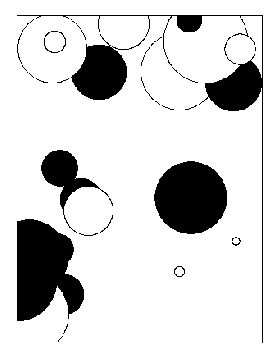
\includegraphics[height=5cm,clip]{Report1.eps}
\caption{演習課題1の画像}
\label{fig:2}
\end{center}
\end{figure}
%----------------------------------------------

\section{考察}
%自分のプログラムの完成度,改善できる点などを書くこと.
\begin{itemize}
\item 白丸を生成する部分と黒丸を生成する部分のコードがほとんど同じになったため、
引数を変えるだけで白丸と黒丸の生成を同じメソッドとしてまとめることができると考えられる。
\item 円の中身を塗りつぶす部分のプログラムで、
左側の円周から右側の円周に向かって中身を塗りつぶしていく
という方法を選んだが、そもそも円周が同じy座標に連続して存在している場合、
この方法では、その円周も塗りつぶしてしまうため、結局、円周を描き直す必要がでてきたため、
この方法で円の中身を塗りつぶすことはあまり効率が良いとは考えられない。
\end{itemize}

\section{感想}
%今回の演習課題1のほか,プログラム課題や
%ロボットTAも含め,授業全般について感想を書くこと.
ロボットTAですぐに答え合わせできるので、プログラムを作ってて楽しいです。


\end{document}

